\documentclass[11pt,a4paper,oneside]{article}

\usepackage[utf8]{inputenc}
\usepackage[T1]{fontenc}
\usepackage{lmodern}
\usepackage[a4paper,margin=21mm,top=23mm,bottom=22mm,headheight=22pt]{geometry}
\usepackage{graphicx}
\usepackage{xcolor}
\usepackage{booktabs,tabularx,array}
\usepackage{fancyhdr}
\usepackage{hyperref}
\usepackage{xurl}
\usepackage{enumitem}
\usepackage{fancyvrb}
\usepackage{titlesec}
\usepackage{caption}
\usepackage{float}
\usepackage[most]{tcolorbox}
\usepackage{microtype}
\usepackage{setspace}
\usepackage{lastpage}

\definecolor{Navy}{HTML}{18334D}
\definecolor{Teal}{HTML}{14877E}
\definecolor{Pale}{HTML}{EDF5F5}
\definecolor{Ink}{HTML}{263746}
\definecolor{Muted}{HTML}{627482}
\definecolor{Amber}{HTML}{A96D18}
\definecolor{AmberPale}{HTML}{FFF5E6}
\definecolor{Red}{HTML}{A83D47}
\definecolor{RedPale}{HTML}{FFF0F1}
\definecolor{Rule}{HTML}{D7E1E6}
\definecolor{CodeBg}{HTML}{F2F5F7}

\hypersetup{
  colorlinks=true,
  linkcolor=Navy,
  urlcolor=Teal,
  citecolor=Navy,
  pdftitle={OpenLain5G User Manual v1.1.9 Candidate},
  pdfauthor={OpenLain5G project},
  pdfsubject={Installation and operation guide for the OpenLain5G local lab},
  pdfkeywords={OpenLain5G, 4G, 5G, Open5GS, user manual}
}
\graphicspath{{images/}}
\setlength{\parindent}{0pt}
\setlength{\parskip}{0.45em}
\setstretch{1.04}
\setlist[itemize]{leftmargin=1.35em,itemsep=0.18em,topsep=0.25em,parsep=0pt}
\setlist[enumerate]{leftmargin=1.55em,itemsep=0.25em,topsep=0.25em,parsep=0pt}
\renewcommand{\arraystretch}{1.22}
\newcolumntype{Y}{>{\raggedright\arraybackslash}X}
\newcolumntype{B}[1]{>{\bfseries\raggedright\arraybackslash}p{#1}}
\newcolumntype{R}[1]{>{\raggedright\arraybackslash}p{#1}}
\captionsetup{font=small,labelfont={bf,color=Navy},textfont={color=Muted},skip=5pt}
\titleformat{\section}{\Large\bfseries\sffamily\color{Navy}}{\thesection}{0.55em}{}
\titleformat{\subsection}{\large\bfseries\sffamily\color{Teal}}{\thesubsection}{0.55em}{}
\titlespacing*{\section}{0pt}{0pt}{0.55em}
\titlespacing*{\subsection}{0pt}{0.8em}{0.25em}

\pagestyle{fancy}
\fancyhf{}
\fancyhead[L]{\sffamily\footnotesize\bfseries\color{Navy} OPENLAIN5G\quad /\quad USER MANUAL}
\fancyhead[R]{\sffamily\footnotesize\color{Muted} v1.1.9 CANDIDATE}
\fancyfoot[L]{\sffamily\footnotesize\color{Muted} Local lab operations guide}
\fancyfoot[R]{\sffamily\footnotesize\color{Muted} \thepage\ /\ \pageref{LastPage}}
\renewcommand{\headrulewidth}{0.4pt}
\renewcommand{\footrulewidth}{0pt}
\renewcommand{\headrule}{\hbox to\headwidth{\color{Rule}\leaders\hrule height \headrulewidth\hfill}}

\newtcolorbox{infobox}{breakable,colback=Pale,colframe=Teal,boxrule=0pt,borderline west={3pt}{0pt}{Teal},arc=1.5mm,left=3mm,right=3mm,top=2mm,bottom=2mm}
\newtcolorbox{cautionbox}{breakable,colback=AmberPale,colframe=Amber,boxrule=0pt,borderline west={3pt}{0pt}{Amber},arc=1.5mm,left=3mm,right=3mm,top=2mm,bottom=2mm}
\newtcolorbox{dangerbox}{breakable,colback=RedPale,colframe=Red,boxrule=0pt,borderline west={3pt}{0pt}{Red},arc=1.5mm,left=3mm,right=3mm,top=2mm,bottom=2mm}
\newtcolorbox{codebox}{breakable,colback=CodeBg,colframe=Rule,boxrule=0.5pt,arc=1.5mm,left=3mm,right=3mm,top=2mm,bottom=2mm}
\newcommand{\cmd}[1]{\texttt{\small #1}}
\newcommand{\tagline}[1]{{\sffamily\footnotesize\bfseries\color{Teal}\MakeUppercase{#1}}}
\newcommand{\manualsection}[2]{\clearpage\section{#1}\label{#2}}
\newcommand{\shotnote}{\textit{Interface reference captured from the local OpenLain5G v1.1.8 browser instance on 7 November 2026.}}

\begin{document}
\thispagestyle{empty}
\vspace*{3mm}
{\color{Teal}\rule{\linewidth}{2.2pt}}\\[11mm]
{\sffamily\bfseries\color{Teal}\large OPENLAIN5G\par}
\vspace{5mm}
{\sffamily\bfseries\color{Navy}\fontsize{33}{38}\selectfont User Manual\par}
\vspace{3mm}
{\sffamily\color{Muted}\Large Install, operate, validate, and safely stop the local lab\par}
\vspace{8mm}
\begin{tcolorbox}[colback=Pale,colframe=Pale,boxrule=0pt,arc=2mm,left=3mm,right=3mm,top=2mm,bottom=2mm]
  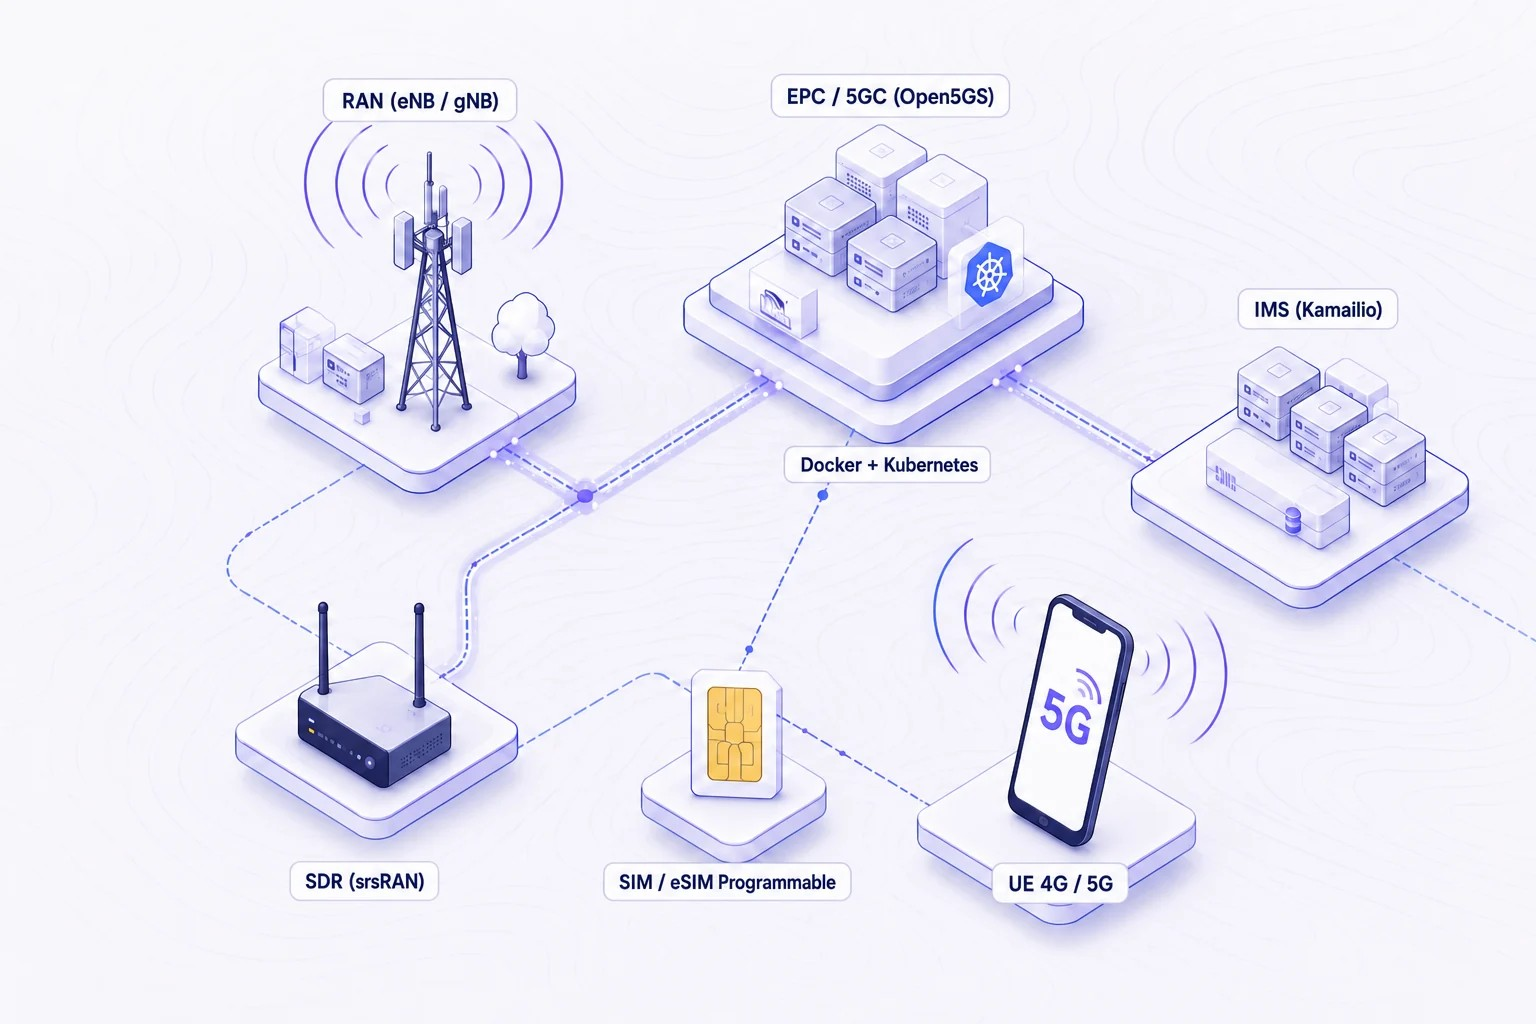
\includegraphics[width=\linewidth,height=9.2cm,keepaspectratio]{hero_topology.jpg}
\end{tcolorbox}
\vspace{5mm}
\begin{minipage}[t]{0.58\linewidth}
  {\sffamily\bfseries\color{Navy}\large A practical guide to the web control plane\par}
  \vspace{2mm}
  {\color{Muted}Use software simulations to learn the workflow. Move to guarded USRP profiles only when the host, radio path, and lab authorization are ready.\par}
\end{minipage}\hfill
\begin{minipage}[t]{0.35\linewidth}
  \begin{tcolorbox}[colback=Pale,colframe=Pale,boxrule=0pt,arc=2mm,left=3mm,right=3mm,top=2mm,bottom=2mm]
    \tagline{Edition}\\
    {\sffamily\bfseries\color{Navy}v1.1.9 candidate}\\[1mm]
    {\small Prepared 7 November 2026}
  \end{tcolorbox}
\end{minipage}
\vfill
{\color{Rule}\rule{\linewidth}{0.5pt}}\\[2mm]
{\small\color{Muted}This manual describes the v1.1.9 source candidate. It is not a release announcement.}
\newpage

\section*{How to use this guide}
\addcontentsline{toc}{section}{How to use this guide}
This guide takes a new operator from a clean checkout to a verified software simulation, then explains subscriber setup, evidence review, optional test-SIM programming, guarded RF operation, and removal. The web interface is the normal way to operate the lab; the CLI installs, starts, and diagnoses it.

\begin{infobox}
\textbf{Start with a simulation.} The 4G LTE and 5G SA software profiles use virtual radio and a simulated UE. They need Docker and a Linux host, but no USRP, antenna, or RF authorization. They validate packet-core and user-plane behavior; they do not establish RF coverage or a physical phone connection.
\end{infobox}

\subsection*{Before you begin}
\begin{itemize}
  \item Use a supported GNU/Linux workstation with Docker Engine and Compose v2 access.
  \item Keep the web interface on loopback at \url{http://127.0.0.1:8080}; do not expose it to an untrusted network.
  \item Allow internet access during installation and first-time image preparation.
  \item Have enough disk space for container images and experiment evidence.
  \item Use only synthetic subscriber credentials for a demonstration unless you control the real test SIM and network.
\end{itemize}

\subsection*{At a glance}
\begin{enumerate}
  \item Clone the repository and run \cmd{./install.sh}.
  \item Start the local web application in operations mode.
  \item Open \textbf{Preparation}, then choose a software profile under \textbf{Scenarios}.
  \item Start the lab, run validation, and review the matching run and logs.
  \item Stop the scenario before starting a different one.
\end{enumerate}

\vspace{1mm}
\begin{center}
\begin{minipage}{0.88\linewidth}
\begin{codebox}
\begin{Verbatim}[fontsize=\small]
git clone https://github.com/guallycanazas/Lain5G.git
cd Lain5G
./install.sh
./lain5g app start --operations --open
\end{Verbatim}
\end{codebox}
\end{minipage}
\end{center}

\clearpage
\subsection*{Contents}
\setcounter{tocdepth}{1}
\tableofcontents
\clearpage

\manualsection{Install and open the web app}{install}
\subsection{Install from a clean checkout}
From a terminal, clone OpenLain5G and run the installer from the repository root:
\begin{codebox}
\begin{Verbatim}[fontsize=\small]
git clone https://github.com/guallycanazas/Lain5G.git
cd Lain5G
./install.sh
\end{Verbatim}
\end{codebox}

The installer prepares host prerequisites, private local configuration, pinned public-profile images, PC/SC and CCID reader support, the SIP lab tool, and first-party Real IMS service images built from the checked-out Dockerfiles. The Real IMS images are built locally; operators do not need to publish them to Docker Hub. Image preparation requires internet access and may take several minutes. The installer displays privileged commands before using them.

To inspect the actions without applying them, run \cmd{./install.sh \mbox{-}\mbox{-}dry-run}. If the installer adds the current account to the Docker group, log out and back in, or run \cmd{newgrp docker}, before starting the app.

At the end, review the host and package-manager summary, dependency and image counts, Docker access, and elapsed time. The installer prints the exact path to its restricted-permission transcript. By default, it is stored here:
\begin{codebox}
\begin{Verbatim}[fontsize=\small]
${XDG_STATE_HOME:-~/.local/state}/lain5g/install-<UTC timestamp>.log
\end{Verbatim}
\end{codebox}
A successful install means tools and images were prepared; it does not mean a profile has been started or validated.

\subsection{Start the application}
\begin{codebox}
\begin{Verbatim}[fontsize=\small]
./lain5g app start --operations --open
\end{Verbatim}
\end{codebox}

Open \url{http://127.0.0.1:8080} if the browser does not open automatically. Operations mode lets the app manage local containers and scenario state. Treat this as administrator-level access to the workstation: use it only on a trusted lab machine. Observation-only mode is available with \cmd{./lain5g app start \mbox{-}\mbox{-}open}; it cannot start or modify scenarios.

\begin{figure}[H]
\centering
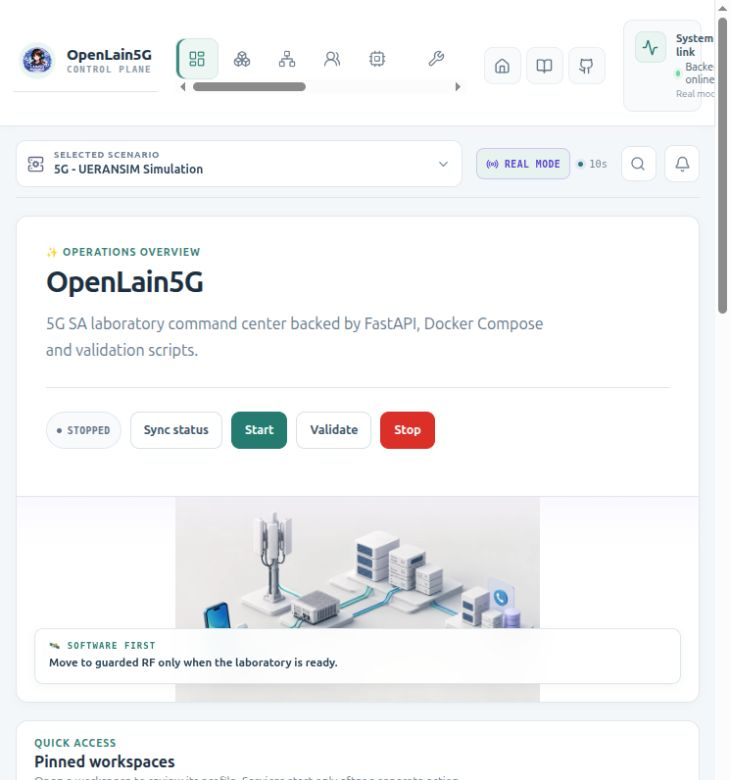
\includegraphics[width=0.67\linewidth]{ui_dashboard.png}
\caption{Dashboard and quick access to the software workspaces. \shotnote}
\end{figure}

\begin{infobox}
The application status in the upper bar is the live connection and version indicator. The dashboard's \textbf{Start}, \textbf{Validate}, and \textbf{Stop} actions control the selected default workspace. A green validation from an earlier run is saved evidence, not proof that services are running now.
\end{infobox}

\manualsection{Choose a profile}{profiles}
Open \textbf{Scenarios} to choose one of the five public workspaces. Pick the software profile first unless the experiment specifically needs physical radio hardware.

\begin{center}
\begin{tabularx}{\linewidth}{B{3.25cm} Y R{4.4cm}}
\toprule
Profile & Use it for & Requirements and scope \\
\midrule
4G LTE Simulation & LTE attach, bearer, UE tunnel, and IP connectivity over virtual ZMQ radio. & Docker, CPU, and TUN device; no USRP or RF. No IMS call testing. \\
4G Guarded LTE RF & A controlled LTE session with the Open5GS EPC and a compatible USRP. & USRP, appropriate UE/SIM, checked RF path, local authorization, and safety gates. \\
5G SA Simulation & 5G registration, PDU session, tunnel, and data ping with UERANSIM. & Docker, CPU, and TUN device; no USRP or RF. No IMS call testing. \\
5G SA Guarded RF & A controlled standalone 5G radio session with Open5GS. & Compatible USRP, UE/SIM, checked RF path, local authorization, and safety gates. \\
5G NSA Guarded EN-DC RF & An LTE anchor with a 5G NR secondary carrier. & Compatible two-chain USRP and UE band combination; both RF paths require their own checks and authorization. \\
\bottomrule
\end{tabularx}
\end{center}

The displayed profile name is intended for operators; its technical ID appears in run reports and CLI commands. The 5G NSA profile uses a shared LTE EPC. Internal VoLTE/VoNR signaling components are not separate public profile entries.

\begin{cautionbox}
Simulation and RF results have different scope. A simulated UE registering successfully is not evidence that a phone received RF or that a commercial UE can attach to a radio.
\end{cautionbox}

\manualsection{Prepare and run a software simulation}{simulation}
\subsection{Prepare the host and profile}
Open \textbf{Preparation} before the first run. Review the host diagnostics and profile image readiness. If components are missing, use \textbf{Prepare missing components} and confirm the operation. Preparation downloads or builds components; it does not start a RAN, UE, or RF transmission.

\begin{figure}[H]
\centering
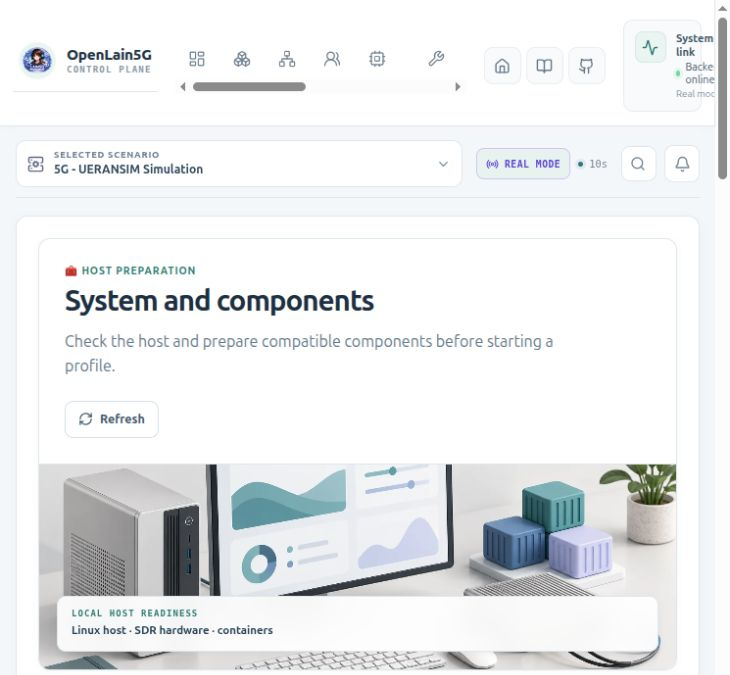
\includegraphics[width=0.49\linewidth]{ui_preparation.png}
\caption{Preparation page. Readiness and diagnostic counts are computed for the current host. Host-specific detail is intentionally excluded from this example. \shotnote}
\end{figure}

For a CLI preflight, use:
\begin{codebox}
\begin{Verbatim}[fontsize=\small]
./lain5g status
./lain5g doctor
./lain5g doctor 5g-sa
./lain5g images list
\end{Verbatim}
\end{codebox}

\subsection{Start, validate, and stop}
\begin{enumerate}
  \item In \textbf{Scenarios}, open \textbf{4G - srsRAN ZMQ Simulation} or \textbf{5G - UERANSIM Simulation}.
  \item Review the profile overview and the \textbf{Preparation} card. Prepare missing components if the page offers that action.
  \item Select \textbf{Start lab} and wait for the startup result. Startup means the requested services were launched; it is not by itself proof that the UE registered.
  \item Select \textbf{Run evidence check} or open \textbf{Validation} and run a fresh check for the selected profile.
  \item Confirm the relevant stages: core readiness, RAN setup, UE registration, bearer/PDU session, tunnel/IP, and data ping.
  \item Review the run created for that attempt. Stop the profile when finished.
\end{enumerate}

The web workspace keeps the launch action, validation, logs, and run report together. The CLI profile IDs are \cmd{5g-sa} and \cmd{4g-lte-sim}; see Section~\ref{cli} for the command reference.

\manualsection{Stop, switch, and preserve evidence}{lifecycle}
Stop the selected scenario from its workspace or dashboard. When starting a different profile, OpenLain5G checks whether another scenario is active; if so, it explains the conflict and asks whether to stop the active profile before continuing. Confirm only when you intend to end that run.

\begin{itemize}
  \item \textbf{Stop scenario} stops the selected scenario services and retains its run and validation evidence.
  \item \textbf{Stop application} stops the web application, monitoring stack, and SIM bridge. It is separate from stopping the profile.
  \item \textbf{App status} and the dashboard show the current live state. A previous report remains available after stop.
  \item Normal stop and profile switching do not delete named Docker volumes or saved run evidence.
\end{itemize}

\begin{codebox}
\begin{Verbatim}[fontsize=\small]
./lain5g scenario status 5g-sa
./lain5g scenario stop 5g-sa
./lain5g app status
./lain5g app stop
\end{Verbatim}
\end{codebox}

\begin{infobox}
Keep the report with the run ID when sharing results. Check the report timestamp and active status before describing a check as current. Validation results summarize what was observed at their run time; they are not a live service monitor.
\end{infobox}

\manualsection{Manage subscribers}{subscribers}
The \textbf{Subscribers} page manages Open5GS subscriber records for the supported RF packet cores. The selected database must be reachable: start the matching core first, then select its profile in Subscribers. A stopped core may make the database appear disconnected or time out; the page does not start that core automatically.

\subsection{Choose a preset}
\begin{itemize}
  \item \textbf{Voice + data} provisions the shared \cmd{internet} and \cmd{ims} service profiles and the voice/data policy defaults used by the lab.
  \item \textbf{Data only} provisions \cmd{internet} only.
\end{itemize}

The subscriber's IMSI, Ki, and OP/OPc must match the test SIM. Authentication values are 128-bit secrets and are not displayed in full in subscriber lists. The UI supplies normal defaults for values such as AMF, SQN, SST, and the default DNN/APN. Use advanced fields only when the SIM or network plan requires a different value. Do not copy a masked value into a new record.

\begin{figure}[H]
\centering
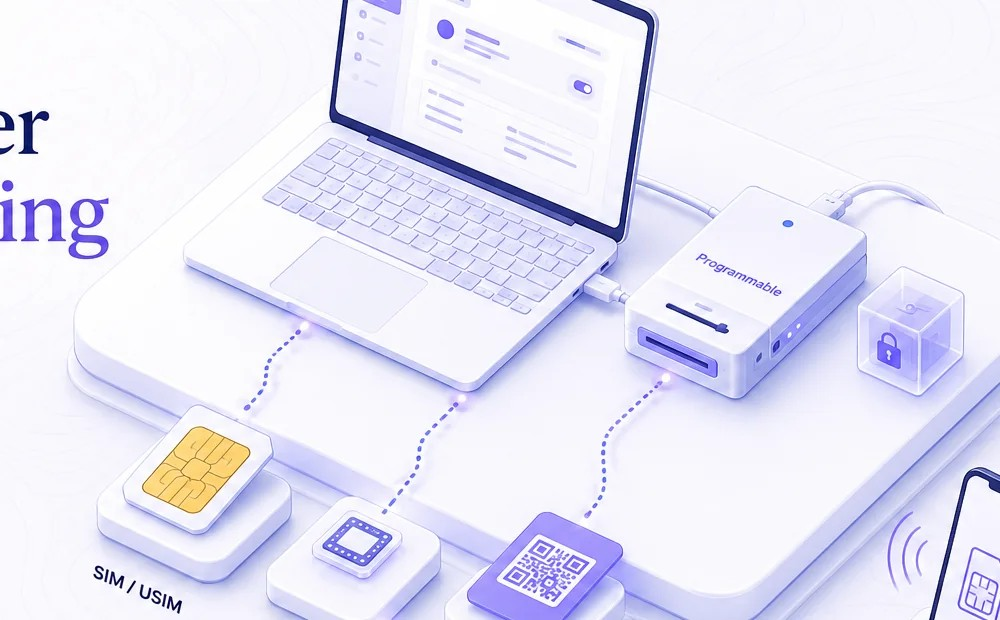
\includegraphics[width=0.42\linewidth]{subscriber_provisioning.jpg}
\caption{Subscriber provisioning illustration used by the web interface. It is an illustration, not a live database screenshot.}
\end{figure}

\begin{cautionbox}
One subscriber identity can be represented in more than one local service database because Open5GS packet-core records and IMS/AuC records serve different functions. Use the same IMSI and matching SIM credentials; the IMS view is not a second person or second phone. A database record does not prove that a UE authenticated.
\end{cautionbox}

\subsection{Create or update safely}
\begin{enumerate}
  \item Select the intended packet-core profile and confirm its connection is ready.
  \item Select \textbf{Create subscriber}, choose \textbf{Voice + data} or \textbf{Data only}, and enter the IMSI and test-SIM credentials.
  \item Review the summary and confirm. Use synthetic values for a demo.
  \item After a UE attempt, use the profile's validation and logs to check registration and session evidence.
  \item Edit or delete records only after confirming the target IMSI and the active profile.
\end{enumerate}

The 5G NSA profile shares the LTE EPC subscriber database. 5G SA uses its own database. The interface routes requests to the selected local profile; it does not accept an arbitrary MongoDB address from the browser.

\manualsection{Program an optional test SIM}{sim}
SIM programming is optional. It writes a physical card and is separate from creating the matching subscriber record.

\subsection{Supported cards and prerequisites}
Connect a PC/SC reader, run the installer, and start the application in operations mode. The page detects sysmoUSIM-SJS1, sysmoISIM-SJA2, and sysmoISIM-SJA5. In this version, only sysmoUSIM-SJS1 is writable; SJA2 and SJA5 are read-only. Unknown cards are not written. The card's ADM1 is required. Do not guess it; failed checks may lock card administration.

\begin{dangerbox}
A card write changes the physical SIM. Verify the reader, card model, MCC/MNC, IMSI, ICCID, Ki, OPc, and ADM1 before confirming. Only program a lab test SIM you are authorized to modify.
\end{dangerbox}

\subsection{Programming sequence}
\begin{enumerate}
  \item Open \textbf{SIM Programmer}, select a reader, and inspect the card before writing.
  \item Enter the network identifiers and the card values; generate fresh synthetic secrets for a lab SIM if needed.
  \item Enter ADM1, acknowledge the write, and confirm in the final dialog.
  \item Wait for the read-back verification. If an operation is interrupted, inspect the card before retrying.
  \item Optionally save an encrypted credential backup. Keep its passphrase separately.
  \item Add the same subscriber credentials in the matching Open5GS core. SIM programming does not create or synchronize the subscriber record.
\end{enumerate}

The optional backup is encrypted in the browser. OpenLain5G does not store the passphrase, and cannot recover the backup if that passphrase is lost. Commercial operator SIMs, eSIM profiles, and changing carrier provisioning are outside this workflow.

\manualsection{Read validation, logs, runs, and metrics}{evidence}
Each page answers a different operator question:
\begin{center}
\begin{tabularx}{\linewidth}{B{3.0cm} Y}
\toprule
Page & What it tells you \\
\midrule
Dashboard & Is the application or a scenario active now? Provides quick status and common actions. \\
Validation & What checks passed, failed, warned, or were not tested in the latest validation report? \\
Runs & Which start/stop/validation events and report belong to this execution? Use the run ID and time. \\
Logs & What recent service output helps explain a startup, shutdown, or network error? Filter by profile, service, level, and text. \\
Metrics & What is the backend and local monitoring stack doing? Runtime dashboards include request, process, scrape, and selected component signals. \\
Troubleshooter & What likely cause and next step match a profile validation or hardware error? It only offers recovery actions implemented for that profile. \\
\bottomrule
\end{tabularx}
\end{center}

\begin{figure}[H]
\centering
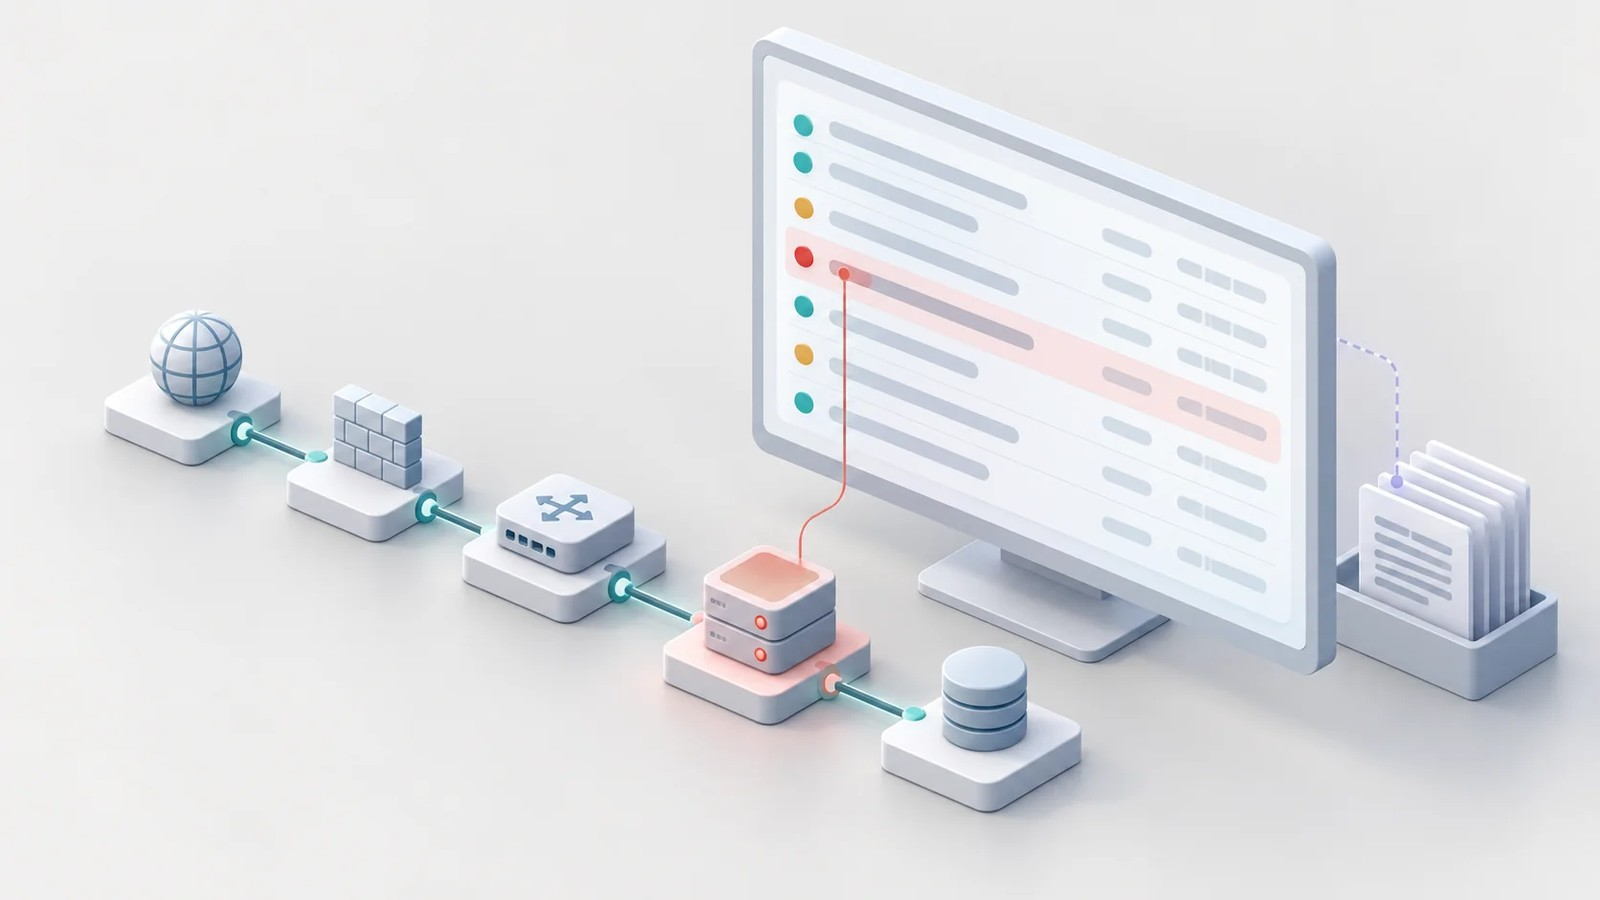
\includegraphics[width=0.48\linewidth]{logs_investigation.jpg}
\caption{Logs investigation illustration used by the web interface.}
\end{figure}

\begin{infobox}
The built-in Grafana dashboards are reached through \textbf{Metrics} in OpenLain5G. Prometheus stores metrics for 15 days; Loki retains collected logs for seven days in local volumes. Application operations mode starts the monitoring stack. The dashboards describe backend/runtime behavior and selected log-derived component activity; they are not SDR spectrum, RF power, or over-the-air UE measurements.
\end{infobox}

\subsection{Make evidence useful}
\begin{enumerate}
  \item Select the same scenario in Validation, Logs, Runs, and Metrics.
  \item Use the newest completed run and record its ID and timestamp.
  \item Compare a failed check with logs from the same profile and time window.
  \item Before exporting logs, remove credentials, IMSIs, phone numbers, private addresses, card/reader details, and RF information.
\end{enumerate}

\manualsection{Troubleshoot common failures}{troubleshooting}
Start with state and evidence before changing configuration:
\begin{codebox}
\begin{Verbatim}[fontsize=\small]
./lain5g status
./lain5g doctor PROFILE
./lain5g scenario status PROFILE
./lain5g scenario validate PROFILE
./lain5g scenario logs PROFILE
\end{Verbatim}
\end{codebox}

\begin{center}
\begin{tabularx}{\linewidth}{B{3.8cm} Y}
\toprule
What you see & First safe checks \\
\midrule
Another scenario is active & Review the active profile and its live status. Stop it only if you intend to end that run; then start the selected profile. \\
Validation is green after Stop & Read the run timestamp. Green is saved evidence; use dashboard state and service inventory for current activity. \\
MongoDB unavailable in Subscribers & Confirm the selected core profile is running and healthy. Select the matching 4G, 5G SA, or shared NSA core. Do not repeatedly submit a write after a timeout. \\
UE did not register or session/ping failed & Read the checks in order: RAN setup, subscription, APN/DNN, session, TUN/IP, then tunnel-bound ping. Open Troubleshooter and the same run's logs. \\
X310 Ethernet link or route failure & Check the cable, selected NIC, link state, local subnet, and route. Use the non-transmitting Hardware check. The app does not rewrite host routes automatically. \\
UHD RFNoC mismatch or management timeout & Compare UHD software and radio FPGA compatibility; inspect Ethernet and the session log. Do not flash firmware or repeat RF start as an automatic retry. \\
Missing image or build & Open Preparation and review the specific component action. Confirm internet access and available disk space; preparing an image does not start the profile. \\
\bottomrule
\end{tabularx}
\end{center}

\begin{infobox}
The Troubleshooter can restart supported simulation services or start an RF profile's core without starting the radio. It will not change host routes, write unknown SIMs, flash a USRP, bypass RF authorization, or erase containers and data.
\end{infobox}

\manualsection{Operate a guarded USRP profile}{rf}
USRP profiles can control radio hardware and may transmit. Follow the local lab's authorization, regulatory rules, channel plan, and written safety procedures. No single frequency, gain, antenna, or attenuation value is correct for every host and jurisdiction.

\begin{figure}[H]
\centering
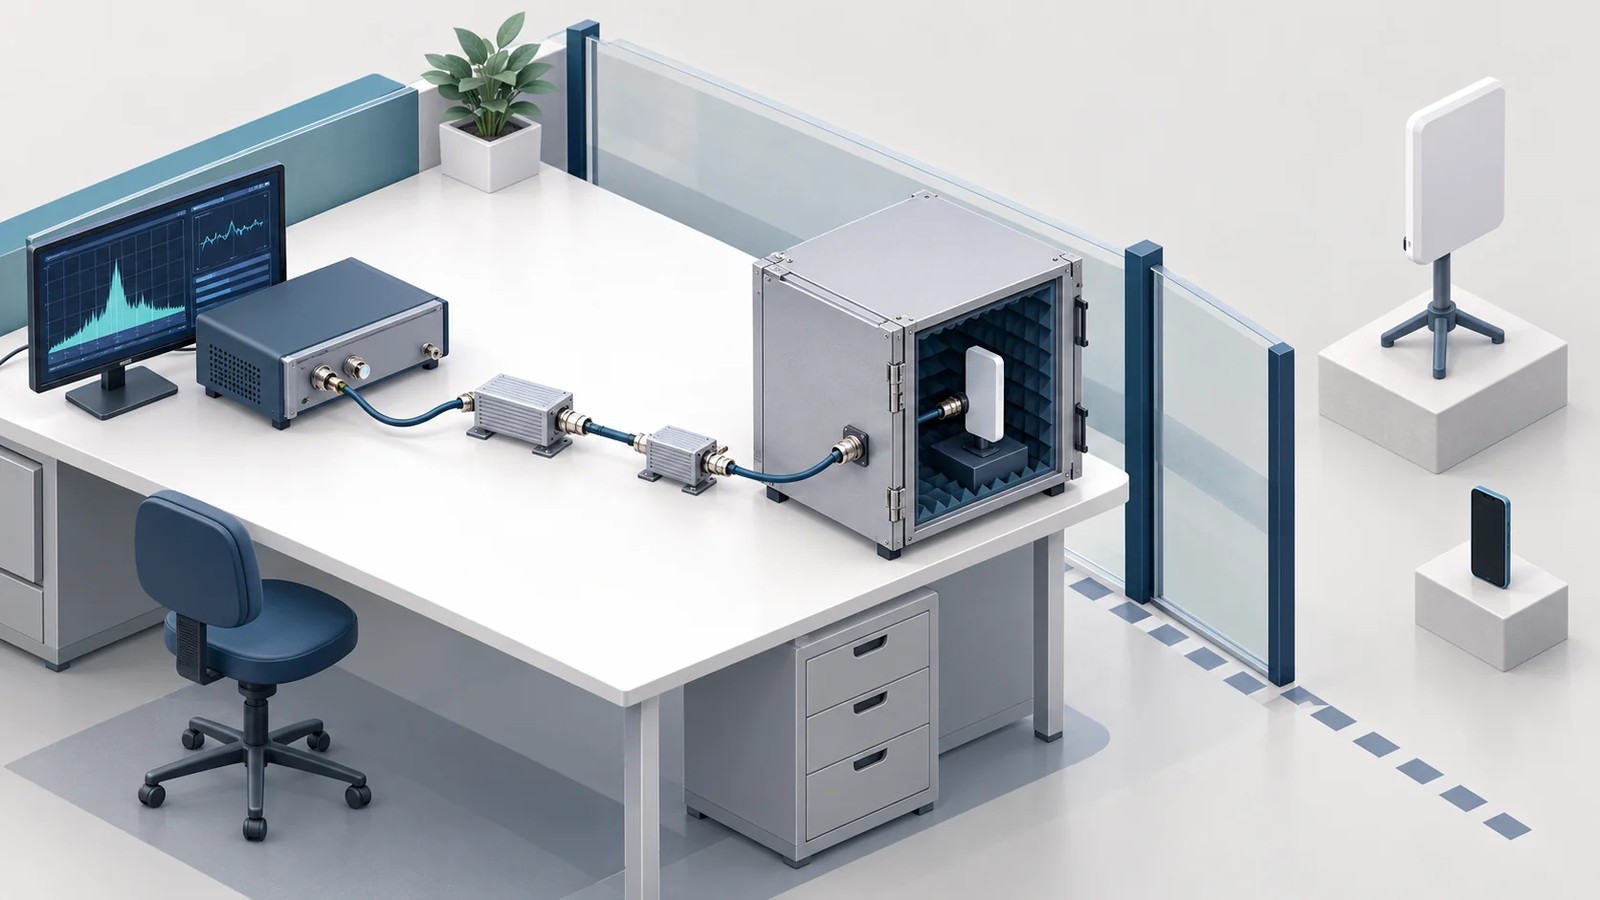
\includegraphics[width=0.50\linewidth]{rf_isolation.jpg}
\caption{Isolated radio laboratory illustration used by the web interface.}
\end{figure}

\subsection{Non-transmitting checks first}
\begin{enumerate}
  \item Confirm the specific profile, compatible USRP model, host UHD build, and FPGA image are supported together.
  \item Check Ethernet link, selected interface, subnet, route, MTU, and device reachability.
  \item Run \textbf{Hardware check} and \textbf{Preflight}. These checks do not transmit.
  \item Confirm the lab setup is cabled or properly shielded, attenuation is measured, and the antenna path is controlled.
  \item Review the band, channel, bandwidth, TX/RX gain, duration, and authorization with the responsible operator.
  \item Confirm the Emergency Stop is accessible and a finite session duration is configured.
  \item Start RF only after the app's checklist and exact confirmation steps pass. Monitor the session and stop if the setup differs from the reviewed plan.
\end{enumerate}

\begin{dangerbox}
A successful software simulation, a green saved validation, or a running container does not mean that RF is authorized or safe. Never bypass a guard, change a route or FPGA image on a troubleshooting guess, or leave RF running unattended.
\end{dangerbox}

\manualsection{CLI reference, updates, and removal}{cli}
\subsection{Everyday commands}
\begin{codebox}
\begin{Verbatim}[fontsize=\small]
./lain5g status
./lain5g app status
./lain5g app logs
./lain5g doctor PROFILE
./lain5g images list
./lain5g scenario status PROFILE
./lain5g scenario validate PROFILE
./lain5g scenario logs PROFILE
./lain5g scenario stop PROFILE
\end{Verbatim}
\end{codebox}

Replace \cmd{PROFILE} with one of these technical profile IDs:
\begin{codebox}
\begin{Verbatim}[fontsize=\small]
4g-lte-sim    4g-lte-x310    5g-sa
5g-sa-x310    5g-nsa-x310
\end{Verbatim}
\end{codebox}
The web interface is recommended for normal operation because it presents the profile state, confirmations, validation, and logs together.

\subsection{Check and change versions}
Use \cmd{./lain5g version}, \cmd{./lain5g version check}, and \cmd{./lain5g version list} to inspect the checkout and available stable tags. Before switching versions, stop scenarios and review the worktree. The manager requires a clean worktree and creates a local backup branch before switching to a tag. To preview a change, use:
\begin{codebox}
\begin{Verbatim}[fontsize=\small]
./lain5g version use v1.1.9 --dry-run
\end{Verbatim}
\end{codebox}

A version switch leaves Git on the selected tag. Keep the backup branch name printed by the command so you can return to local work.

\subsection{Remove components or data}
Use the staged uninstaller and preview the scope before applying it. Normal removal stops and removes the selected Compose containers and networks while preserving named volumes, images, local configuration, evidence, and the checkout.
\begin{codebox}
\begin{Verbatim}[fontsize=\small]
./lain5g uninstall --scope app --dry-run
./lain5g uninstall --scope all --dry-run
./lain5g uninstall --scope all
\end{Verbatim}
\end{codebox}

A complete removal with \cmd{\mbox{-}\mbox{-}purge-all} also deletes OpenLain5G-labeled data and the checkout, including uncommitted local changes. Back up any subscriber data and run evidence you need. The command shows a preview and requires the exact interactive phrase \cmd{BORRAR OPENLAIN5G COMPLETAMENTE}; \cmd{\mbox{-}\mbox{-}yes} cannot bypass this confirmation. Do not use \cmd{docker system prune} as an OpenLain5G removal method.

\manualsection{Edition and manual updates}{edition}
\begin{infobox}
\textbf{Manual edition: v1.1.9 candidate.} The repository source candidate is v1.1.9 and has not been published. The browser was available locally for documentation work, but the running interface identified itself as v1.1.8. Captured UI screens are therefore visual references for navigation and layout; they are not evidence that v1.1.9 was running or validated.
\end{infobox}

The manual edition should advance with each software release. Update the user-facing steps, requirements, profile catalog, screenshots, and troubleshooting notes whenever a release changes what an operator sees or does. A code change that does not alter user workflows does not require rewriting every page. Keep the manual source and its PDF together under the same version directory so the source used to produce an edition can be reconstructed.

For a published release, regenerate or verify browser captures against that exact release before describing them as current. The application header shows the running version. The cover, PDF metadata, source folder, release notes, and download filename should all identify the same manual edition.

\subsection*{Documentation and support}
\begin{itemize}
  \item Project documentation: \url{https://github.com/guallycanazas/Lain5G/tree/main/docs}
  \item Source repository and issue tracker: \url{https://github.com/guallycanazas/Lain5G}
  \item Installation details: \cmd{docs/installation.md}
  \item Subscriber details: \cmd{docs/subscribers.md}
  \item RF safety details: \cmd{docs/rf\_safety.md}
  \item SIM Programmer details: \cmd{docs/sim\_programmer.md}
\end{itemize}

\vfill
\begin{center}
{\color{Rule}\rule{0.8\linewidth}{0.5pt}}\\[2mm]
{\small\color{Muted}OpenLain5G is a local research and training lab. Follow the rules and safety procedures that apply to your site.}
\end{center}

\end{document}
